% Version 02

\documentclass[a4paper]{article}
\pagestyle{empty}
\usepackage{amssymb}
\usepackage{amsmath}
\usepackage{graphicx}
\usepackage{epstopdf}
\usepackage[left=1.0in,top=1.0in,right=1.0in,bottom=2.5in]{geometry}
\setlength{\textwidth}{6.27in}
\setlength\topmargin{0.0in}
\setlength\headheight{0.5in}
%\setlength{\topmargin}{0.25in}
%\setlength\headheight{0.25in}

\usepackage{fancyhdr,lastpage}
\pagestyle{fancy}
\chead{A Hybrid CFD/MD Simulation on Multi-physical Fluid System using SAGA and BigJob, Page \thepage~of \pageref{LastPage}}
\fancyhead[L]{}
\fancyhead[R]{}
\cfoot{A Hybrid CFD/MD Simulation on Multi-physical Fluid System using SAGA and BigJob, Page \thepage~of \pageref{LastPage}}


\begin{document}
\begin{center}


%%%%% TITLE %%%%%
\textbf {\large \bf A Hybrid CFD/MD Simulation on Multi-physical Fluid System 
using SAGA and BigJob}
%\doublespacing
\vspace{14pt}

%%%%% AUTHORS %%%%%
\textbf {\normalsize \hspace{0.6 in} Shantenu Jha$^1$, Nayong Kim$^1$, Soon-Heum Ko$^1$, Abhinav Thota$^1$, \newline
Joohyun Kim$^1$ and Dimitris Nikitopoulos$^2$}

\vspace{12pt}

%%%%% AFFILIATIONS %%%%%
\normalsize { \hspace{0.6 in} $^1$Center for Computation and Technology, \newline Louisiana State University, Baton Rouge, LA 70803, USA}

\normalsize {\hspace{0.6 in} $^2$Mechanical CityEngineering Department, \newline Louisiana State University, Baton Rouge, LA 70803, USA}

\vspace{12pt}

\end{center}

%%%%% MAIN TEXT %%%%%
A hybrid CFD/MD approach~\cite{Nie:2004},~\cite{Yen:2007} is a latest simulation method which adopts the continuum hypothesis in capturing the macroscopic features of a flowfield and resolves intermolecular effects on interfaces of different materials. CFD (Computational Fluid Dynamics) could accurately predict flow properties on conventional moderate/large size fluid domains, but is intrinsically impossible to reflect the characteristics of surrounding solid materials: MD (Molecular Dynamics) guarantees more accurate solution in that it also considers collision between fluid particles as well as interaction with solid particles, while its huge amount of computation time makes this method hard to solve a large scale system. It means that these conventional methods have risks in solving a flowfield where solid boundary��s viscous effect is dominant and the scale is sufficiently large in view of particle dynamics (bigger than nanometer level). These fluid systems can only be analyzed by solving particle interaction near the wall through molecular dynamics and applying a continuum approach on far field region. As is seen in Figure 1, the hybrid approach accurately describes strong interaction between solid elements and fluid particles near the wall and conducts efficient simulation in the far field follows the continuum approach.
Conducting this coupled simulation requires a lot of cautions in view of simulation performance, though code development can be easily done by implementing a hybrid scheme in existing CFD and MD simulation tools - in this simulation, an in-house incompressible CFD code~\cite{Lee:2006} and LAMMPS MD simulation package (http://lammps.sandia.gov) were used - and letting these tools communicate with each other. As CFD and MD codes have frequent communications, (e.g., the CFD code conducts data exchange in every iteration) they should start concurrently though they are recognized as separate packages in the scheduler. Users' account loss is inevitable in conventional queuing systems except when sufficient CPUs are idling, as the first running job has to wait its counterpart to follow. Even in cases with sufficient available resources, a user still experiences the unnecessary waste of computing time because of load imbalance between two simulation tools. As the performance of each tool changes with computing resource and problem size, re-adjustment of allocated resources to each task according to their performance is required during the simulation. However, as two codes are submitted as independent jobs, flexible CPU allocation change between these coupled tools is impossible. Thus, the best way in conventional job submission system would be to find a site with sufficient resource pool and submit two jobs with optimal number of processors according to the pre-test data on performance of each tool in that facility with the same problem size.
Above hardships motivated us to use SAGA (the Simple API for Grid Applications)~\cite{Jha:2008} and the BigJob abstraction~\cite{Jha:2009}. SAGA is designed to deal with distributed infrastructure explicitly and it supports application-level functionality/interface for distributed applications. BigJob abstraction denotes a container task where a number of subtasks can run in pre-defined schedule with specified number of processors whether or not they are coupled. As depicted in Figure 2, designed BigJob architecture for the hybrid CFD/MD simulation consists of SAGA, SAGA glide-in framework and application framework. SAGA is closely connected with other middlewares such as Globus Toolkit (http://www.globus.org) and local schedulers and, bridges the gap between infrastructure and application by providing job control and file management functions in easy-to-use passion. SAGA glide-in framework constitutes the basic pattern of BigJob abstraction. It manages the BigJob submission, actual simulation of subtasks and promotes the re-launch of subtasks. The application framework is composed of two high-end simulation tools, application manager and load balancing module. By submitting a BigJob and specifying application components, the application manager enables the synchronous start of CFD and MD codes. When these two applications paused after producing checkpointing data and performance profile, the application manager re-adjusts processor allocation to each subtask by the help of load balancing module and it eliminates the load imbalance between two application codes.
The essential improvement of BigJob abstraction in this application lies in the existence of load balancing module. In former replica exchange test, a bunch of small tasks with similar problem size were scheduled to run on the BigJob, leaving the requirement of load balancing among subjobs. On the other hand, the current simulation consists of two tightly-coupled large-scale tasks and load balancing between two application components is the core of current simulation, as discussed above. To achieve load balancing, we have implemented a simple load balancing function by the help of time checker in application codes. During the simulation, each application code returns its own simulation time. Assuming that each code has the ideal parallel performance, the load of each task would be the multiplication of their running time and number of processors used. Then, load balancing module re-adjusts resources inversely proportional to their presumed load. Considering every parallel code has different scalability, we can accomplish the load balance by a trial-and-error approach of above function.
We are under implementation of the application manager component and would be testing three different BigJob scenarios to verify the performance of our implementation on tightly-coupled simulations. To see the performance enhancement due to the dynamic execution, we will run one BigJob simulation which contains CFD and MD tasks and check the change of assigned number of processors to each task. The same coupled simulation will be tried by applying two BigJob simulations in the same resource to show the benefit of BigJob abstraction in acquiring maximal available computing resource and, the same test would be done on heterogeneous systems to investigate the influence of multiple sites on the performance of BigJob. These test scenarios could be explained by the schematic on two BigJob submissions in Figure 3. When the first BigJob is allocated, two application codes run with predefined number of processors in each task. During the simulation, application framework changes the processor allocation according to load balancing function and would follow the optimal distribution. When the next BigJob is added to the running simulation, two BigJob resources are fully allotted to simulation codes and it repeats the same load balancing procedure.



\vspace{12pt}

%%%%% REFERENCES %%%%%
\begin{thebibliography}{99}
\bibitem{Nie:2004}
X. B. Nie, S. Y. Chen, W. N. E and M. O. Robbins,
\newblock "A Continuum and Molecular Dynamics Hybrid Method for Micro- and Nano-Fluid Flow,"
\newblock {\em J. Fluid Mech.}, 500, pp. 55-64, 2004

\bibitem{Yen:2007}
T. H. Yen, C. Y. Soong and P. Y. Tzeng,
\newblock "Hybrid Molecular Dynamics-Continuum Simulation for Nano/Mesoscale Channel Flow,"
\newblock {\em Microfluid Nanofluid}, 2007

\bibitem{Lee:2006}
Jung-Sang Lee, Chongam Kim and Kyu Hong Kim
\newblock "Design of Flapping Airfoil for Optimal Aerodynamic Performance in Low-Reynolds Number Flows,"
\newblock {\em AIAA Journal}, 2006

\bibitem{Jha:2009}
Shantenu Jha, Yaakoub El-Khamra, and Joohyun Kim,
\newblock "Developing Scientific Applications with Loosely-Coupled Sub-tasks,"
\newblock in {\em Computational Science - ICCS 2009}, G. Allen, J. Nabrzyski, E. Seidel, G.D. van Albada, J. Dongarra, P.M.A. Sloot (Eds.), Lecture Notes in Computer Science 5544, pp.641-650, 2009

\bibitem{Jha:2008}
A. Luckow, S. Jha, J. Kim, A. Merzky, and B. Schnor
\newblock Adaptive Replica-Exchange Simulations
\newblock {\em Royal Society Philosophical Transactions A} (to appear, 2009)
\end{thebibliography}

\vspace{12pt}

%%%%% FIGURES %%%%%

%================================================================
%  Add new figure (Figure 1) here
%================================================================
%\begin{figure}
%\centering
%\includegraphics[width=5.0in]{Image1.eps}
%\caption{CFD/MD Coupled Simulation on Channel Flow - Now Yet Included}
%\end{figure}
%================================================================

\begin{figure}
\centering
\includegraphics  [scale=0.65]{Image2.eps}
\caption{Architecture of the BigJob Abstraction for Hybrid CFD/MD Approach}
\end{figure}

\begin{figure}
\centering
\includegraphics [scale=0.6]{Image3.eps}
\caption{The Scenario of Load-balanced Coupled Simulation with Two BigJob Abstraction}
\end{figure}

\noindent 

\end{document}


